\documentclass[border=10pt]{standalone}
\usepackage{tikz}
\usetikzlibrary{calc}

\begin{document}
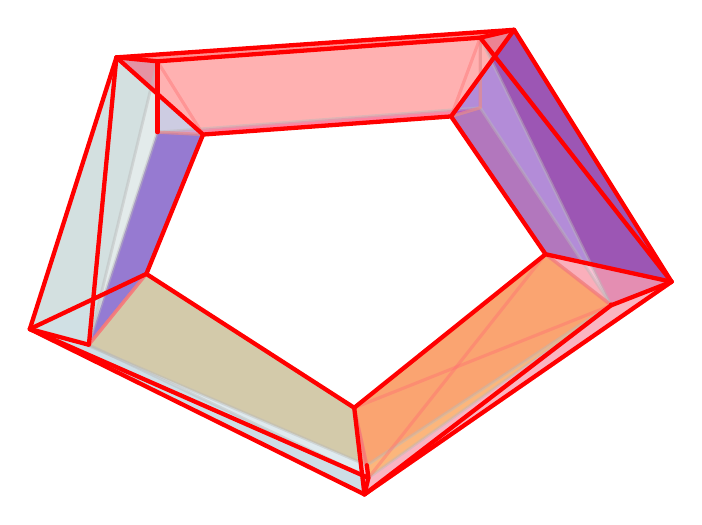
\begin{tikzpicture}[line join=round, line cap=round, x=1cm, y=1cm]

% Front outer pentagon vertices
\coordinate (A1) at (1.10,5.00);
\coordinate (B1) at (6.15,5.35);
\coordinate (C1) at (8.15,2.15);
\coordinate (D1) at (4.25,-0.55);
\coordinate (E1) at (0.00,1.55);

% Front inner pentagon vertices
\coordinate (A2) at (2.20,4.02);
\coordinate (B2) at (5.35,4.25);
\coordinate (C2) at (6.55,2.50);
\coordinate (D2) at (4.12,0.55);
\coordinate (E2) at (1.48,2.25);

% Rear/depth outer pentagon vertices visible through the transparent faces
\coordinate (A3) at (1.62,4.95);
\coordinate (B3) at (5.72,5.25);
\coordinate (C3) at (7.38,1.85);
\coordinate (D3) at (4.30,-0.34);
\coordinate (E3) at (0.75,1.35);

% Rear/depth inner pentagon vertices visible through the transparent faces
\coordinate (A4) at (1.62,4.05);
\coordinate (B4) at (5.72,4.36);
\coordinate (C4) at (7.38,1.86);
\coordinate (D4) at (4.28,-0.18);
\coordinate (E4) at (0.74,1.34);

\tikzset{
  mainedge/.style={red, line width=1.55pt},
  deedge/.style={red!55, line width=1.15pt, opacity=.45},
  hidedge/.style={gray!55, line width=1.05pt, opacity=.45}
}

% Back and side facets first: the transparent 3D thickness of the ring
\fill[teal!45!gray!35, opacity=.43]   (E1) -- (A1) -- (A3) -- (E3) -- cycle;
\fill[violet!55!blue!45, opacity=.48] (A3) -- (A1) -- (A2) -- (A4) -- cycle;
\fill[red!55!pink, opacity=.43]       (A1) -- (B1) -- (B3) -- (A3) -- cycle;
\fill[magenta!35!violet, opacity=.50] (B1) -- (C1) -- (C3) -- (B3) -- cycle;
\fill[orange!65!red!35, opacity=.42]  (C1) -- (D1) -- (D3) -- (C3) -- cycle;
\fill[green!40!blue!35, opacity=.40]  (D1) -- (E1) -- (E3) -- (D3) -- cycle;

% Inner wall/depth facets around the hole
\fill[violet!55!blue!55, opacity=.47] (A2) -- (A4) -- (E4) -- (E2) -- cycle;
\fill[red!35!magenta, opacity=.38]    (A2) -- (B2) -- (B4) -- (A4) -- cycle;
\fill[orange!50!red!45, opacity=.43]  (B2) -- (C2) -- (C4) -- (B4) -- cycle;
\fill[magenta!45!pink, opacity=.39]   (C2) -- (D2) -- (D4) -- (C4) -- cycle;
\fill[teal!38!green!35, opacity=.35]  (D2) -- (E2) -- (E4) -- (D4) -- cycle;

% Front colored facets of the pentagonal band
\fill[red!42!pink, opacity=.54]       (A1) -- (B1) -- (B2) -- (A2) -- cycle;
\fill[purple!45!blue, opacity=.45]    (B1) -- (C1) -- (C2) -- (B2) -- cycle;
\fill[magenta!34!pink, opacity=.47]   (C1) -- (D1) -- (D2) -- (C2) -- cycle;
\fill[cyan!35!gray!45, opacity=.47]   (D1) -- (E1) -- (E2) -- (D2) -- cycle;
\fill[teal!40!gray!35, opacity=.45]   (E1) -- (A1) -- (A2) -- (E2) -- cycle;

% Small differently colored front subdivisions visible in the reference
\fill[orange!70!yellow, opacity=.42]  (C2) -- (D2) -- (D3) -- (C3) -- cycle;
\fill[blue!45!violet, opacity=.38]   (E2) -- (A2) -- (A4) -- (E4) -- cycle;
\fill[brown!45!orange, opacity=.28]  (D2) -- (E2) -- (E4) -- (D4) -- cycle;

% Hidden/rear subdivision edges across the transparent facets
\draw[hidedge] (A3) -- (B3) -- (C3) -- (D3) -- (E3) -- cycle;
\draw[hidedge] (A4) -- (B4) -- (C4) -- (D4) -- (E4) -- cycle;
\draw[hidedge] (A3) -- (A4);
\draw[hidedge] (B3) -- (B4);
\draw[hidedge] (C3) -- (C4);
\draw[hidedge] (D3) -- (D4);
\draw[hidedge] (E3) -- (E4);
\draw[hidedge] (A1) -- (A3);
\draw[hidedge] (B1) -- (B3);
\draw[hidedge] (C1) -- (C3);
\draw[hidedge] (D1) -- (D3);
\draw[hidedge] (E1) -- (E3);
\draw[hidedge] (A2) -- (A4);
\draw[hidedge] (B2) -- (B4);
\draw[hidedge] (C2) -- (C4);
\draw[hidedge] (D2) -- (D4);
\draw[hidedge] (E2) -- (E4);

% Red internal/depth edges and subdivisions visible on the facets
\draw[deedge] (A3) -- (A4) -- (A2);
\draw[deedge] (B3) -- (B4) -- (B2);
\draw[deedge] (C3) -- (C4) -- (C2);
\draw[deedge] (D3) -- (D4) -- (D2);
\draw[deedge] (E3) -- (E4) -- (E2);
\draw[deedge] (B3) -- (B2);
\draw[deedge] (C3) -- (C2);
\draw[deedge] (D3) -- (D2);
\draw[deedge] (E3) -- (E2);
\draw[deedge] (A3) -- (A2);
\draw[deedge] (C2) -- (D3);
\draw[deedge] (C3) -- (D2);
\draw[deedge] (D2) -- (D4);
\draw[deedge] (E2) -- (E4);

% Front red outline and hole outline
\draw[mainedge] (A1) -- (B1) -- (C1) -- (D1) -- (E1) -- cycle;
\draw[mainedge] (A2) -- (B2) -- (C2) -- (D2) -- (E2) -- cycle;

% Main radial/front connecting edges
\draw[mainedge] (A1) -- (A2);
\draw[mainedge] (B1) -- (B2);
\draw[mainedge] (C1) -- (C2);
\draw[mainedge] (D1) -- (D2);
\draw[mainedge] (E1) -- (E2);

% Prominent rear red silhouette/depth edges
\draw[mainedge] (A1) -- (A3) -- (B3) -- (B1);
\draw[mainedge] (B3) -- (C1);
\draw[mainedge] (C1) -- (C3) -- (D1);
\draw[mainedge] (D1) -- (D3) -- (E1);
\draw[mainedge] (E1) -- (E3) -- (A1);
\draw[mainedge] (A3) -- (A4);
\draw[mainedge] (C3) -- (C4);
\draw[mainedge] (D3) -- (D4);

\end{tikzpicture}
\end{document}
